\casesection{Bed slope effect (1)}
\label{case:e02-f22-c17}

\paragraph*{Purpose}

The purpose of this validation case is to examine  bed slope effect in influencing the bed load transport of D-Flow FM-sed-mor . A straight channel flow simulations with minor longitudinal slope and trench in middle of the channel has been prescribed. The test case number is e02-f22-c17.
\paragraph*{Linked claims}
%\begin{itemize}
%	\item
The bed slope influences the direction of bed load transport as expected, according to the comparison executed between three simulations (with structured and unstructured grid of FM and D3D) of the test case. However, the magnitude of bed load transport is not same in the three simulation this may require further investigation.
% almost the same result compare to Delft3D software. 
%\end{itemize} 
\paragraph*{Approach}
Three simulations have been prepared
%\begin{enumerate}
%	\item 
and all the input is specified using D-Flow flexible mesh (FM)-sed-mor module and Delft3D4 model.
%\end{enumerate}

\paragraph*{Model Description}
The test case concern a straight channel flow with a various transverse slopes and a constant roughness factor under equilibrium flow conditions. A discharge $Q$ equal to 2 m$^3$/s is prescribed as upstream boundary condition. The longitudinal bottom slope $i_b$ is prescribed to be $0$. The transverse slope is 0.22  (see \ref{fig:net}). The width of the channel is 1.6 m and the corresponding bed level difference at the left and right bank are 0.35 m a. The Ch\'ezy friction coefficient $C$ is set to 60 m$^{1/2}$/s. The downstream boundary condition is water level set to 0.17 m.

The default parameters in the morphological setup are mainly used.Nevertheless, in the following part important related setup of morphology and sediment files used are described as follows:

In addition, an important related setup to morphology file and sediment file used in these testcass are described as follows:
\begin{itemize}
	\item[$\bullet$] Sediment file <*.sed>:
\end{itemize}
\begin{verbatim}
[Sediment]
SedTyp           = bedload               # Must be "sand", "mud" or "bedload"
SedDia           = 5.0e-004              # [m] Median sediment diameter (D50)
TraFrm           = 1
Name             = #Engelund-Hansen (1967)#
ACal             = 0.6
RouKs            = 0.08
\end{verbatim}
$SedTyp$ is bedload,
sediment transport equation is Engelund-Hansen (1967),
sediment size ($D_{50}$) is equal to 0.5 mm.
\begin{itemize}
	\item[$\bullet$] Morphology file <*.mor>:
\end{itemize}
The morphology update $ MorUpd$ and bed composition update  $CmpUpd$ are off and
$AlfaBs$ is equal to 1 and the bed slope effect is computed by Koch and Flokstra (1980).

\begin{figure}[h!]
	\begin{center}
		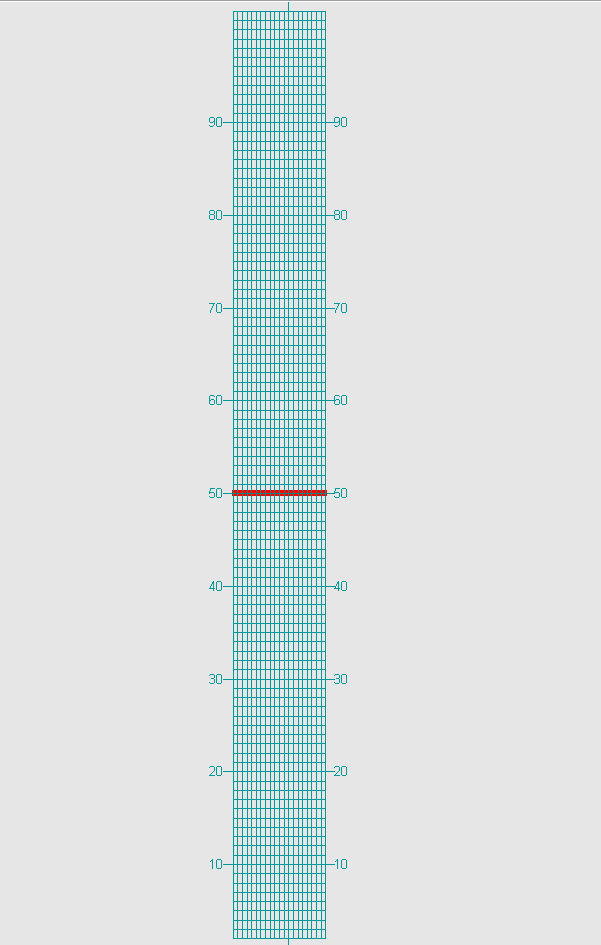
\includegraphics[width=0.7\columnwidth] {figures/the-cross-sectionLocation.PNG}
	\end{center}\caption{c17 the channel grid used and the cross-section where the result is illustrated (with red color)}
	\label{fig:net}
\end{figure}

\begin{figure}[h!]
	\begin{center}
		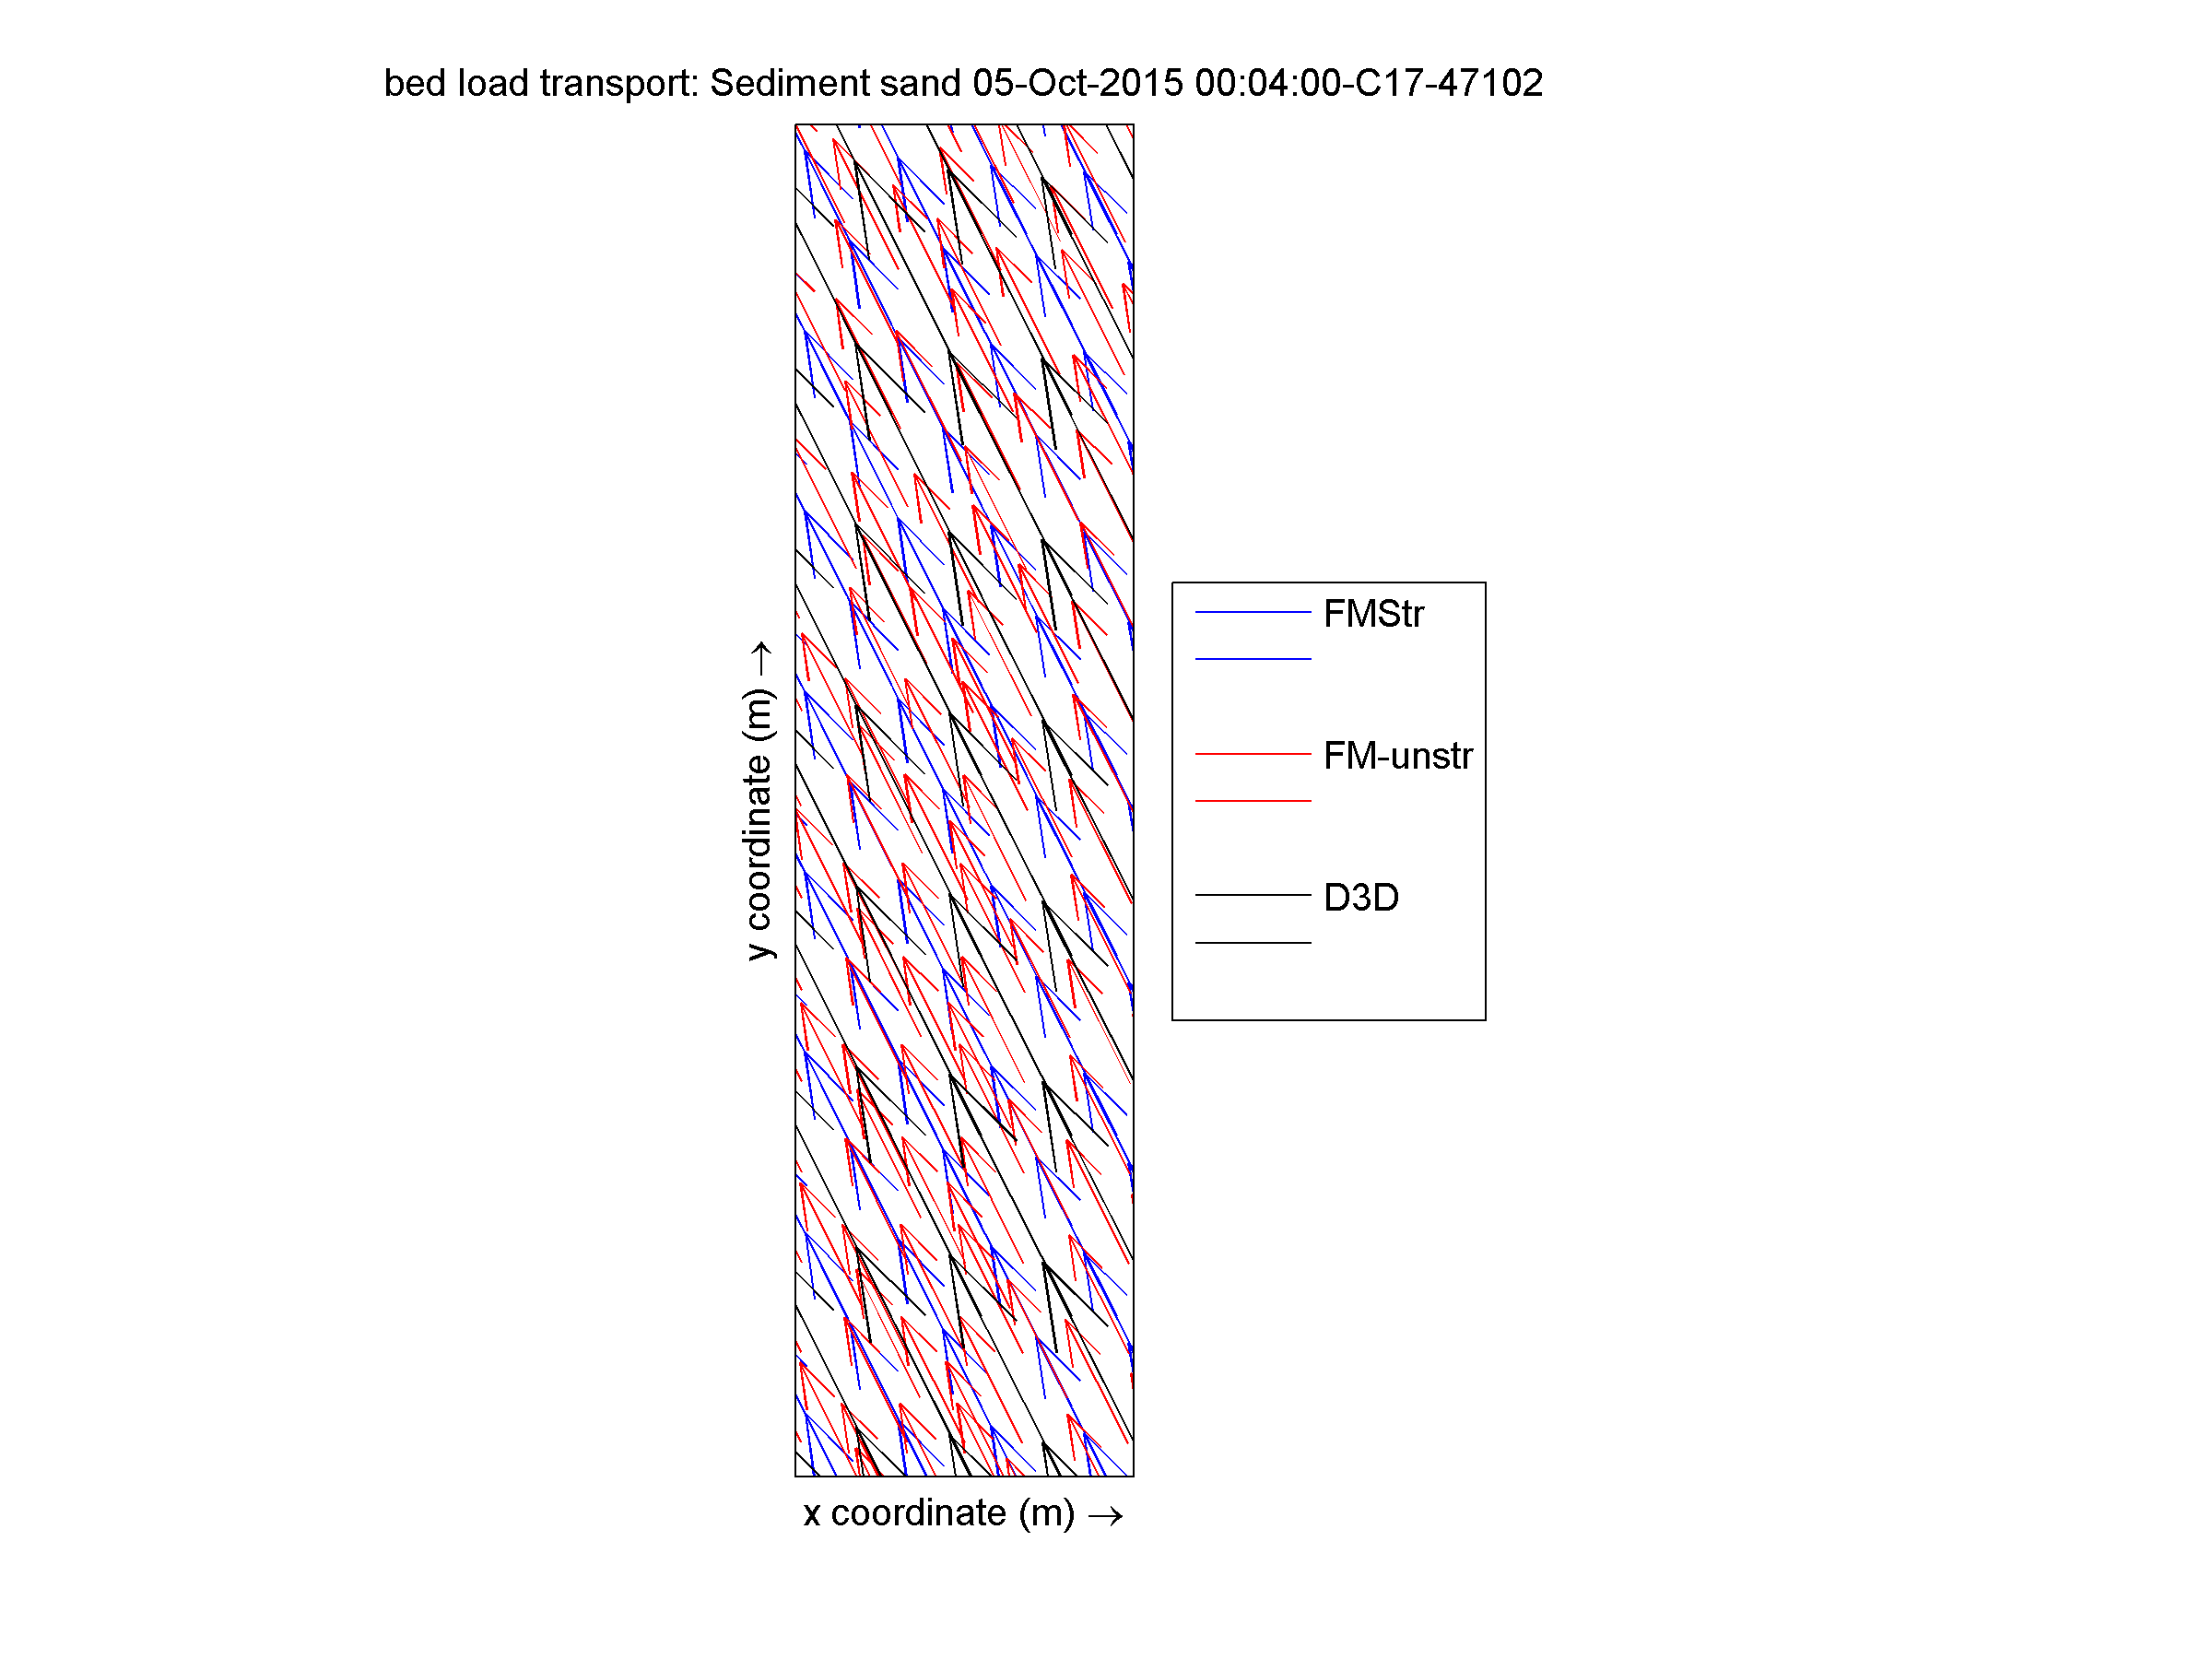
\includegraphics[width=0.9\columnwidth] {figures/C17-bed-Slope-Effect-VectorMap.png}
	\end{center}\caption{C17-The direction of the bed load transport}
	\label{fig:vectors}
\end{figure}

\begin{figure}[h!]
	\begin{center}
		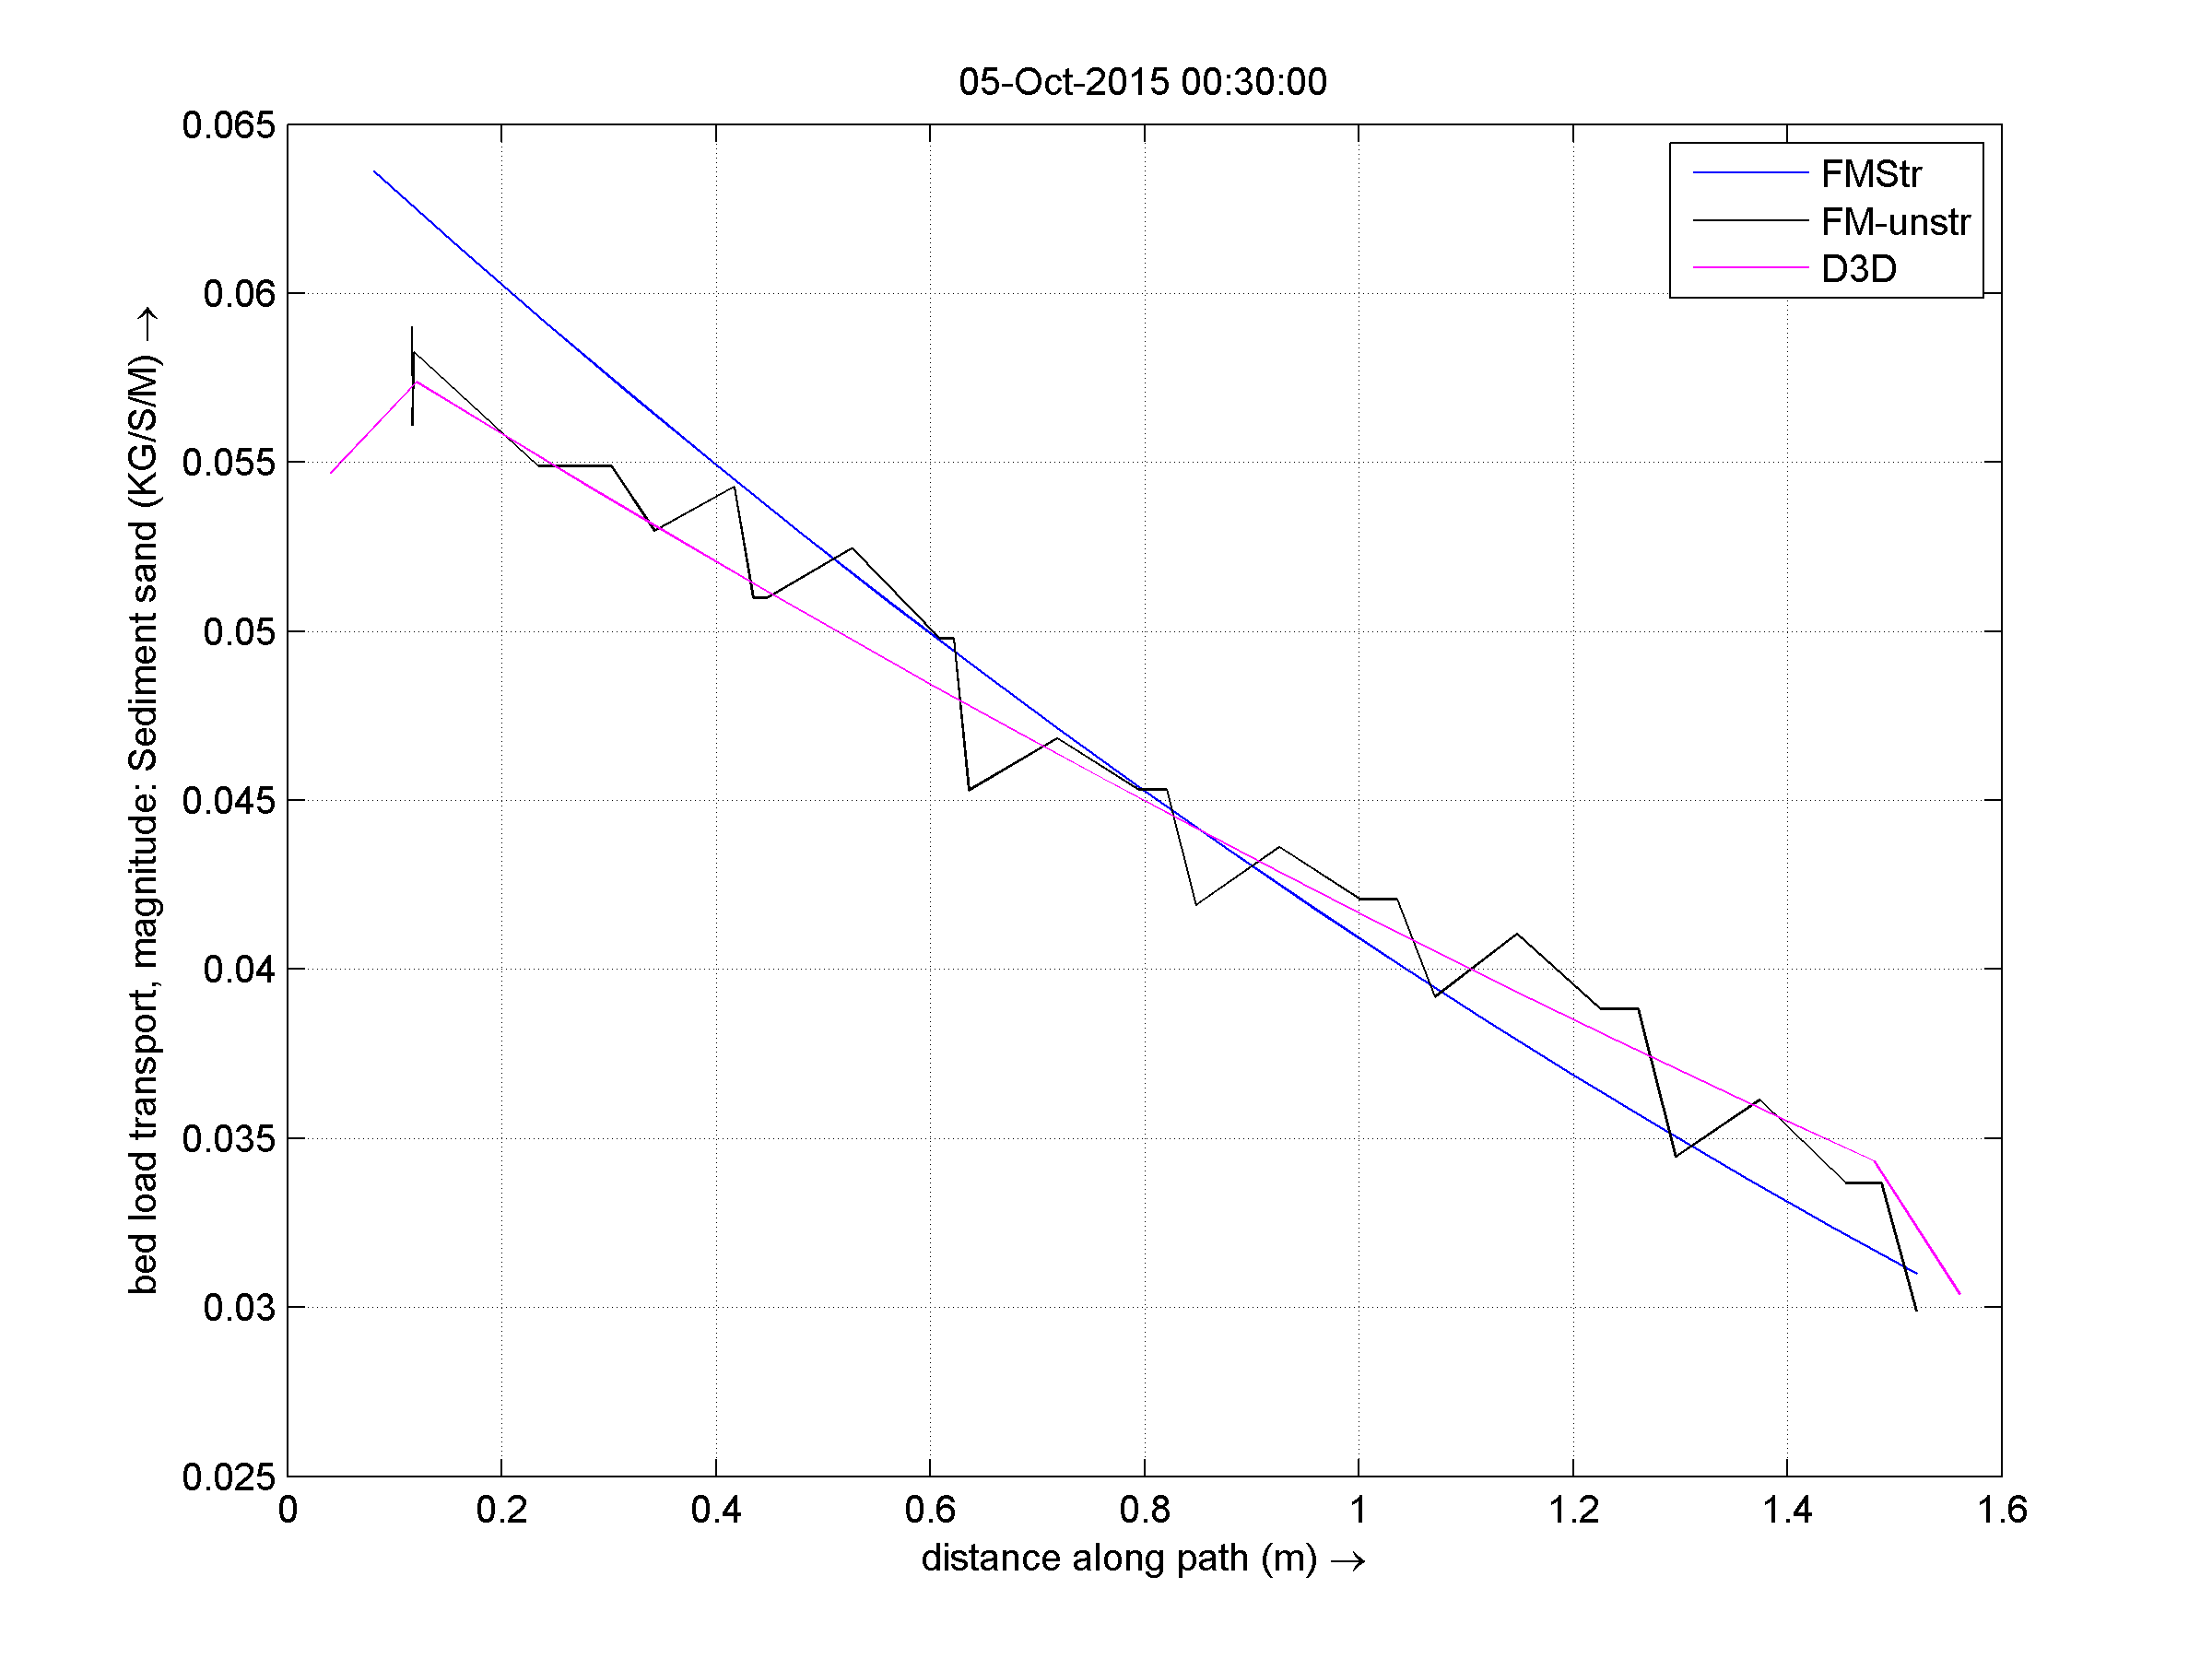
\includegraphics[width=0.7\columnwidth]{figures/C17-bed-Slope-Effect47116.png}
	\end{center}\caption{Bed load transport magnitude}
	\label{fig:mag}
\end{figure}

\paragraph*{Results}

The results show that the direction of bed load transport of the structured and unstructured grid is almost similar to Delft3D (see fingure \ref{fig:vectors}). However, the magnitude of bed load tranport is not fully the same if we compare the three simulation as shown in figure \ref{fig:mag}.

\paragraph*{Conclusion}
The result shows that direction fo bed load transport of FM is comparable with Delft3D4. The magnitude of the bed load  require more investigation.
\paragraph*{Version}
This test has been carried out using the following software versions:
\begin{itemize}
	
	\item[$\bullet$] dflow-fm-x64-1.1.188.47116 for flexible Mesh. 
	\item[$\bullet$] FLOW2D3D Version 6.01.07.3574 for Delft3D4
	
\end{itemize}

%------------------------------------------------------------------------------

